\chapter{Megvalósítás}

\section{Grafikák elkészítése}

Mielőtt, hogy nekiláttam a grafikai elemek létrehozásának, inspirációként szolgáltak az interneten elérhető rajzolási stílusok és csempekészletek. Az alapja és mintája a saját rajzaimnak a Ninja Adventure Tileset volt, amelyet Pixel-boy készített.\cite{NAT}

\subsection{Grafikus szerkesztő}

Fontos kiemelni, hogy egy "pixelart" rajz stílusról beszélünk az esetemnben, ezért kerestem olyan rajzprogramot választanom amely minden igényemet kielégíti és könnyen kezelhető tapasztalatlan grafikusok számára is. A kiválaszott program az Aseprite volt, ebbe készítettem minden játékban megtalálható grafikát. \cite{Aseprite}

\begin{figure}[H]
    \centering
    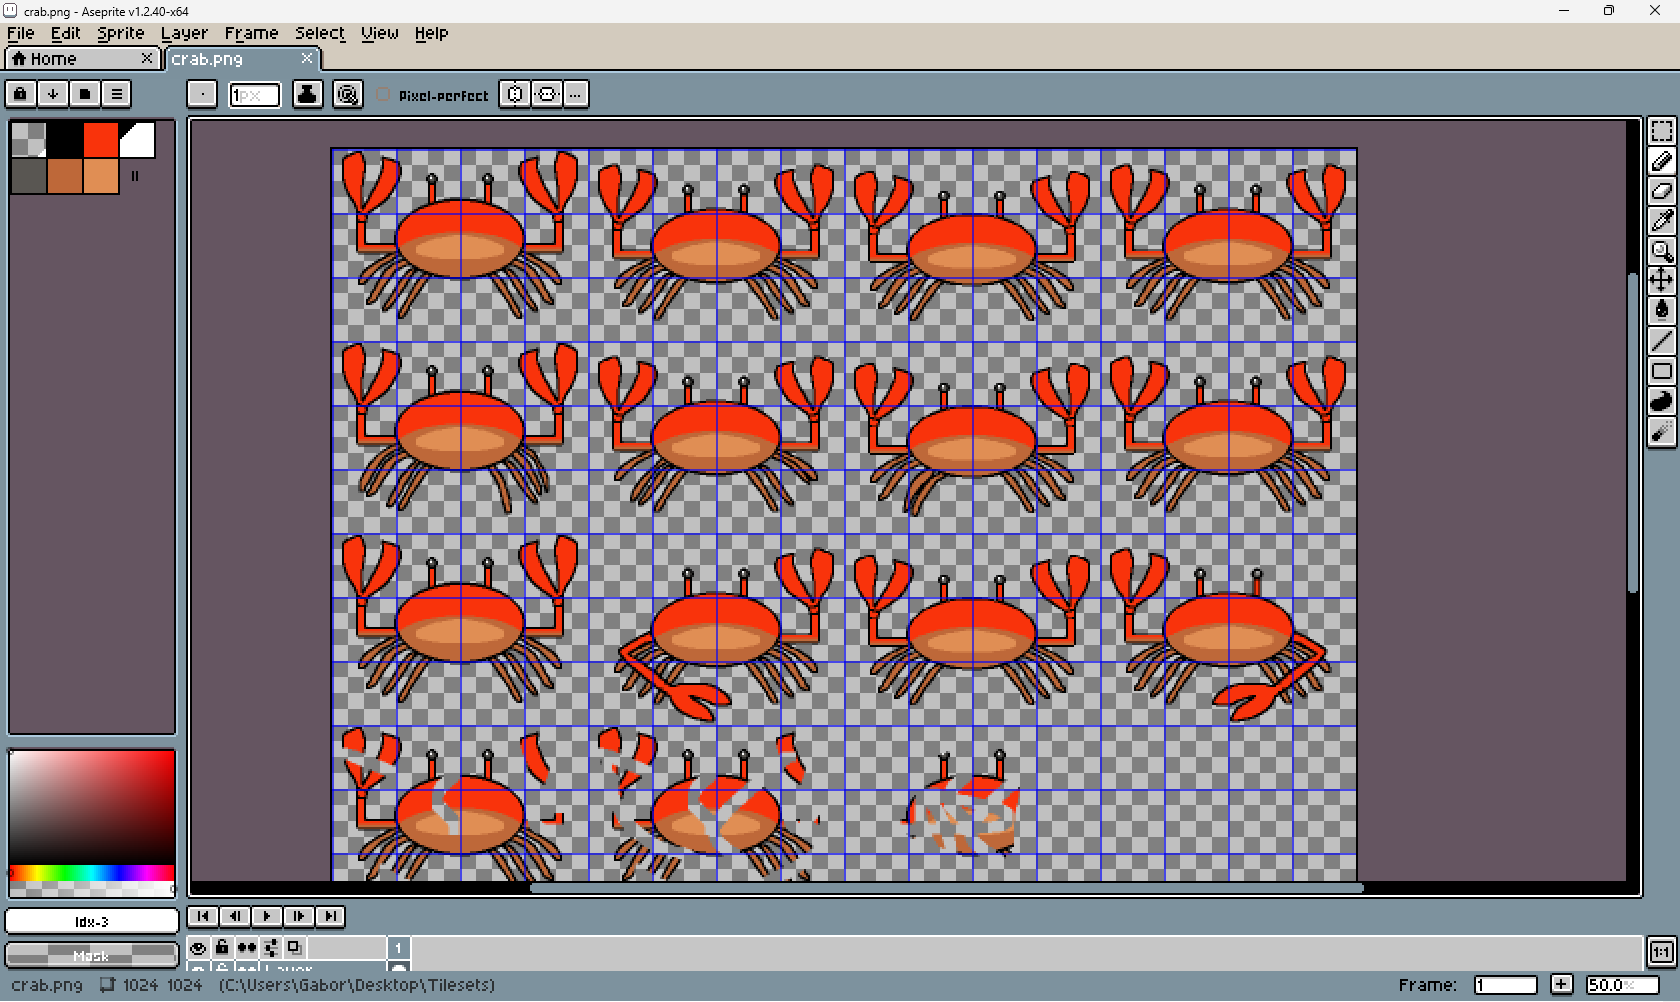
\includegraphics[width=14.0truecm]{images/Aseprite.png}
    \caption{Aseprite}
    \label{fig:Aseprite}
\end{figure}


\subsection{Rajzok elkészítése}

A rajzok elkészítése két fő részből állt, a pálya tervezéséből és a karakterek valamint a környezet kialakításából. A pálya tervezéséhez a korábban említett Ninja Adventure Tileset szolgált mintaként, melyből az összes pálya elemét saját kezűleg rajzoltam meg. A karakterek és környezet rajzainak elkészítésénél pedig meglévő rajzokat használtam inspirációként, és ezeket egészítettem ki saját kreatív ötleteimmel.

\subsubsection{Pálya}
A pályaelemek létrehozásánál kiemelkedően fontos volt figyelnem arra, hogy a csempék harmonikusan illeszkedjenek egymáshoz, ezáltal kellemes és összefüggő látványt teremtve.

\subsubsection{Entitások}
Karakterek, és szörnyek megtervezése annyiban tért el, hogy ott figyelni kellett az animációra is, hiszen élethű mozgást szerettem volna utánozni. Egy ilyen mozgás animáció 4-6 képből áll, amelyeket egymás után lejátszva érhető el a kívánt hatás. Illetve mivel 4 különböző irányba tudnak haladni ezek az entitások ezért 4 különböző animációt kellett elkészítenem, amelyeket a játék során a karakter irányának megfelelően tudtam lejátszani.



\section{Pálya megtervezése}

\subsection{Tiled}
\label{subsec:Tiled}
A pálya megtervezéséhez a Tiled-et \cite{Tiled} választottam ami egy népszerű térképszerkesztő szoftver, amelyet játékfejlesztők használnak a 2D-s játékok pályáinak tervezésére és szerkesztésére. A Tiled egy nyílt forráskódú program, így ingyenesen elérhető és széles körben használt az indie játékfejlesztők körében.

Ez a szoftver lehetővé teszi a felhasználók számára, hogy könnyen létrehozzanak és testreszabjanak térképeket, amelyeket különböző játékkeretrendszerekbe integrálhatnak. A Tiled számos funkciót kínál, mint például csempekészletek használata, rétegek kezelése, objektumok és kollíziók definiálása, valamint az exportálás különböző formátumokban, például CSV vagy TMX (Tiled Map XML).

Az egyszerű és intuitív felhasználói felülete miatt a Tiled ideális eszköz a játékfejlesztők számára, akik részletes és részletekre is figyelő térképeket szeretnének készíteni játékaikhoz. Az XML alapú TMX formátum kompatibilis a legtöbb játékmotorral, így a Tiled segítségével készült térképek könnyen beilleszthetők a fejlesztési folyamatba.


\subsection{Tervezés}

Kiemelkedően fontos volt a pálya elemeit különböző rétegekre szétválasztani, ezáltal megkönnyítve a fejlesztést és az egyes részek kezelését. A háttér szolgálatában álló csempéket például két rétegre osztottam: az egyikre a talajszintet, a másikra pedig a talajon megtalálható növényzetet helyeztem el. Ezt a két réteget együttesen exportáltam PNG formátumban, amelyet a játékban háttérképként fogok használni.Fontos megjegyezni, hogy a két háttér réteget nem mentettem külön CSV fájlba. Ennek oka az, hogy ezek a rétegek olyan elemeket tartalmaznak, amelyek statikusak és nincs velük semmiféle interakció a játék során. 

Van még egy fontos réteg amik akadályként szolgálnak a játékos számára (Lásd 4.2. ábra piroskörvonal), ezeket a rétegeket a játékos nem tudja átlépni, ezáltal a játékmenetet befolyásolják.  

Lettek még rétegek létrehozva az objektumok számára, minden típúsú objektumot külön rétegen helyeztem el, így könnyen kezelhetőek és nem kell a kódban szűrést alkalmazni a különböző típusú objektumok használatakor.

\begin{figure}[H]
    \centering
    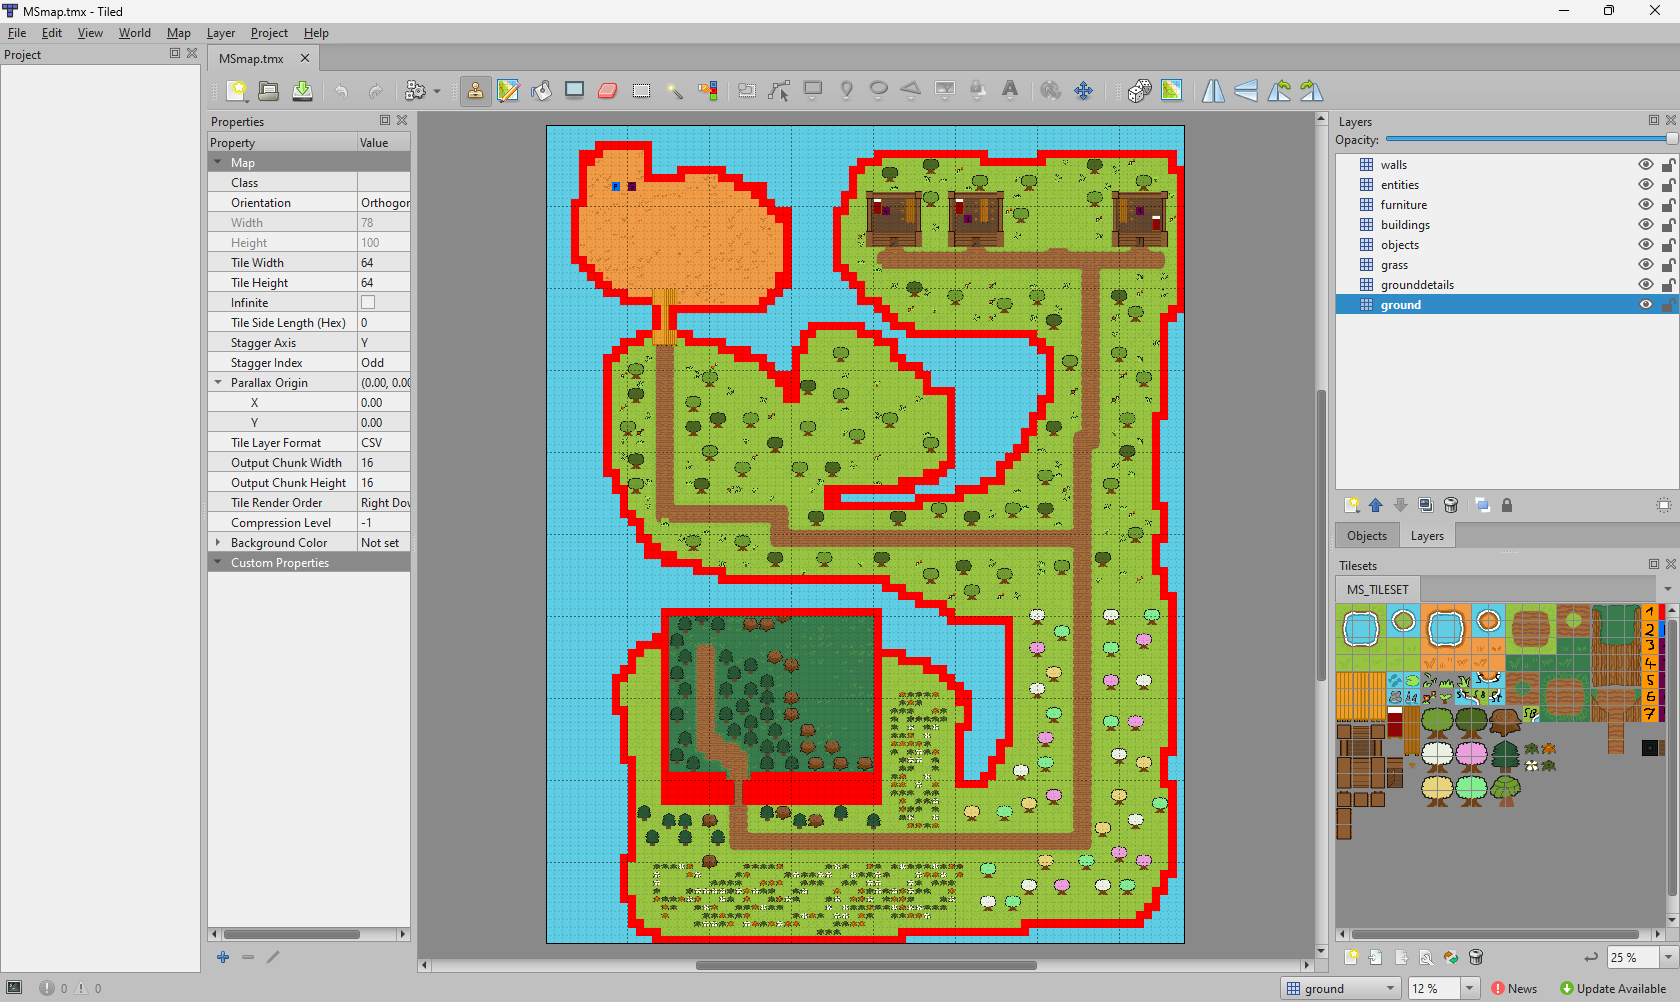
\includegraphics[width=14.0truecm]{images/Tiled.png}
    \caption{Tiled}
    \label{fig:Tiled}
\end{figure}




\section{Definiált osztályok bemutatása}
A következő szekcióban a definiált osztályok kerülnek bemutatásra.


\subsection{Settings}
Ennek az osztálynak a fő célja a beállítások kezelése egy játékban vagy alkalmazásban. Az osztály tartalmazza az alapértelmezett beállításokat, mint például a játékablak méretét, a hangerejét és egyebeket. Az osztály segítségével ezeket a beállításokat be lehet tölteni és menteni egy JSON fájlba.

Az osztályban található statikus osztályváltozók az alapértelmezett beállításokat tárolják, és a program különböző részeiben felhasználhatók. Az osztályban található statikus osztályváltozók az alapértelmezett értékeket tárolják, és a program különböző részeiben felhasználhatók, anélkül hogy az osztály példányt kellene létrehozni belőle, így könnyen hozzáférhetőek.

Az osztály további adatokat is tartalmaz, például hangokat, grafikákat, karaktereket, ellenségeket, lövedékeket és fegyvereket. Mindezek az adatok részletezik a játékbeli objektumok tulajdonságait.

Az osztály emellett definiálja a felhasználói felület színeit és stílusait, amelyek a játék megjelenítéséhez használatosak. Ezek a színek és stílusok segítenek a felhasználói felület személyre szabásában.


\subsection{Game osztály}
Ez az osztály felelős a játék főciklusának végrehajtásáért, ami az egész játék működésének alapját képezi. Amikor a játék elindul, az alkalmazás példányosítja ezt az osztályt, és ennek a főciklusnak a futása irányítja a játékmenetet.

A 4.1. programkód részletesen bemutatja, hogyan kell megvalósítani ezt a főciklust, amely a játék lényegét adja. Ebben a kódban kezeljük a játék fő eseményeit, és gondoskodunk arról, hogy minden szükséges műveletet végrehajtsunk a játék folyamán.

Amennyiben a menürendszer visszaadja a menuenums.GAME értéket, az azt jelenti, hogy a játékot választottuk a menüből, és belépünk a játék főciklusába. Itt történik minden, a játékmenet során szükséges frissítés, eseménykezelés és kirajzolás. Itt szabjuk meg a képfrissítés mértékét is a 'self.clock.tick(Settings.FPS)' sorral, amely a másodpercenként kirajzolandó képkockák számát határozza meg.

Ez az osztály tehát létfontosságú szerepet játszik abban, hogy a játék működése zökkenőmentes legyen, és a kódban látható példa segítségével könnyen megérthető, hogyan történik mindez.


\begin{python}[caption={Játék főciklusa},label=py:főciklus]
    def run(self):

        while True:
            elif self.state == menuenums.GAME:
                if self.game_handler is None:
                    Sounds.play_loop('main')
                    self.game_handler = GameHandler(
                        self.user, self.save_parameters)
                for event in pygame.event.get():
                    if event.type == pygame.QUIT:
                        pygame.quit()
                        sys.exit()
                self.screen.fill(Settings.WATER_COLOR)
                self.game_handler.run()
                pygame.display.update()
                self.clock.tick(Settings.FPS)
\end{python}



\subsection{UserAuth}
Ez az osztály kezeli a regisztrációhoz és a bejelentkezéshez kapcsolódó folyamatokat. Ilyen folyamat többek között a felhasználói felület megjelenítése, de a tartalom ellenőrzés és hibakezelés is.

\subsection{MainMenu}

A játéknak elengedhetetlen része a főmenü, ami a bejelentkezés után válik elérhetővé a felhasználók számára. Biztosítok a játékosoknak offline azaz internet nélküli játszási lehetőséget, ilyenkor regisztráció és bejelentkezés nélkül használni lehet a játékot.
A főmenüben három menüpont található meg, az új játék létrehozása, meglévő mentés betöltése, illetve a beállítások. (lásd. 4.3. ábra.)   



\begin{figure}[H]
    \centering
    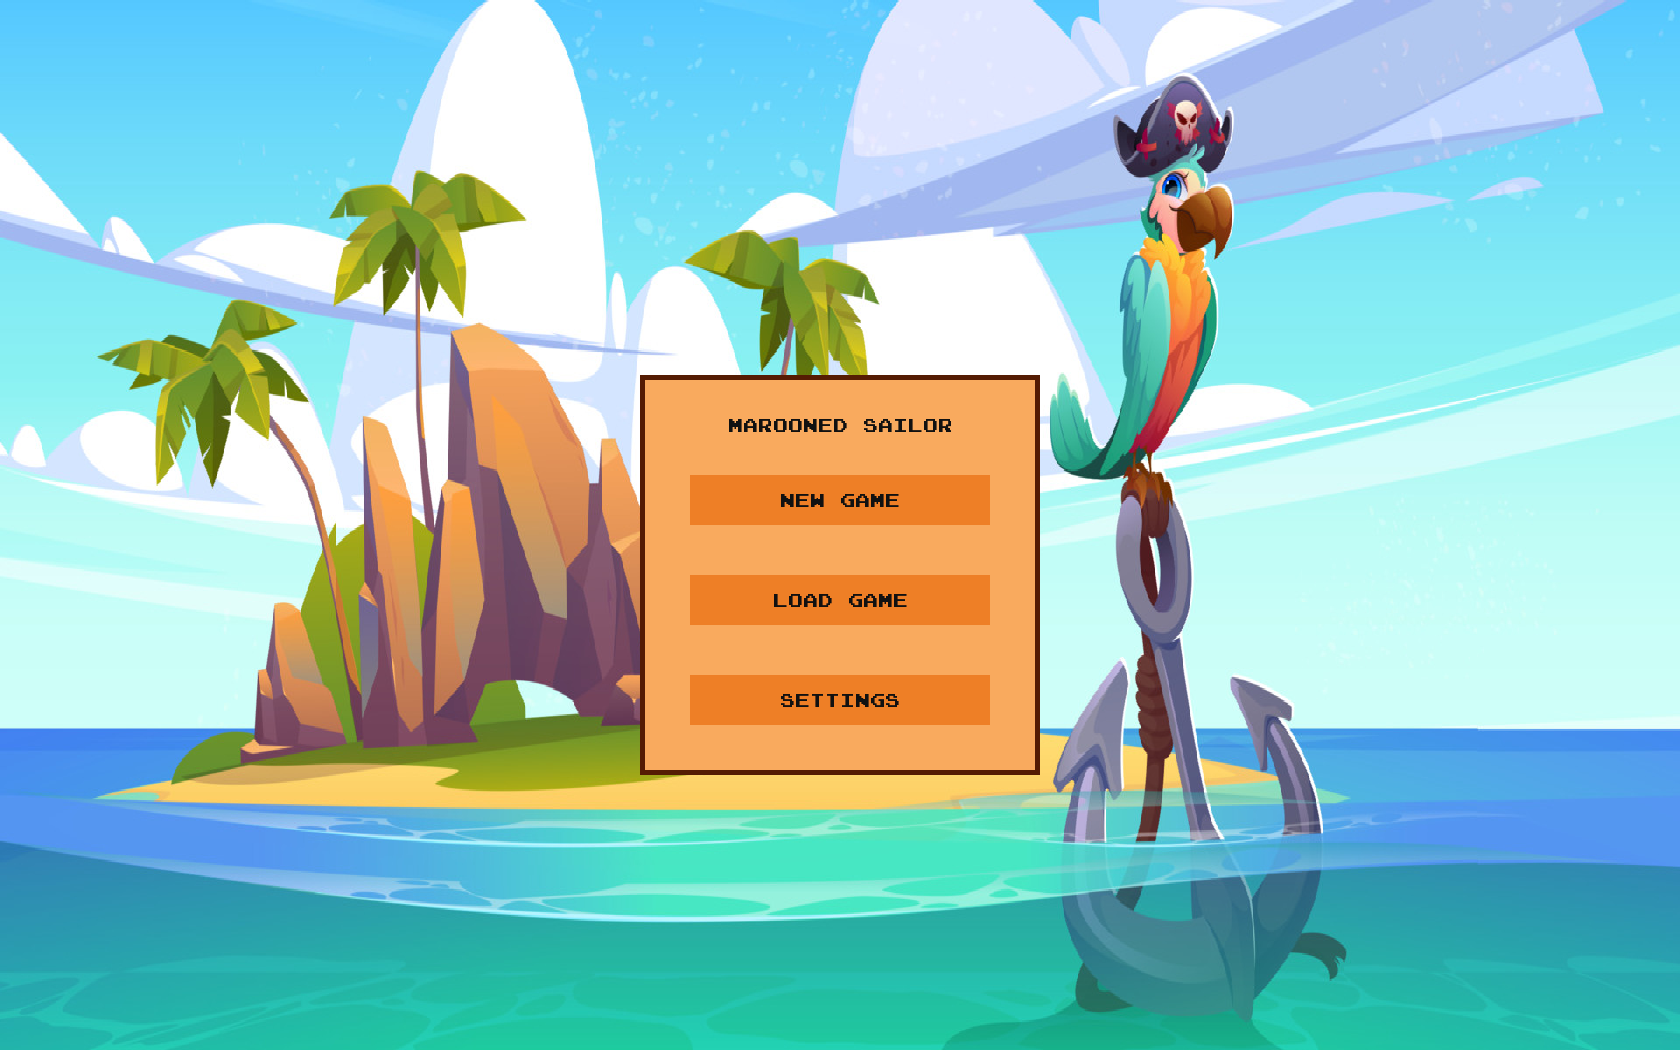
\includegraphics[width=15.0truecm]{images/mainmenu.png}
    \caption{Főmenü}
    \label{fig:Főmenü}
\end{figure}



\subsection{NewGameMenu}
Az új játék menüpont kiválasztása után a játékosnak meg kell adni a karakterének a nevét, illetve választhat különböző karakter kinézet közül. Ha be van jelentkezve a játékos, akkor van lehetősége nehézségi szintet is választani.
A nehézségi szint annyiban különbözik, hogy a "normal" módban, ha elfogynak a játékos életpontjai, akkor a játék folytatódik tovább, újraéled egy bizonyos helyen. Viszont, ha a "challange"  módot választja akkor három funkcióval bővül a játékmenet. Az első ilyen funkció, hogy ha elfogy a játékos életereje akkor véglegesen meghal a karakter, és nem lesz lehetősége tovább folytatni azzal a bizonyos karakterrel a játékot. A második plusz funkció, hogy az összes küldetés teljesítése esetén a játék újrakezdődik amely azt eredményezi, hogy a szörnyek erősödnek, és nagyobb kihívás lesz újra végigvinni az összes küldetést. Illetve tartalmaz egy ranglista menüpontot, amely jelzi a legügyesebb játékosok hányszor tudták a "challange" mód használatával végigvinni az összes küldetést. 

\begin{figure}[H]
    \centering
    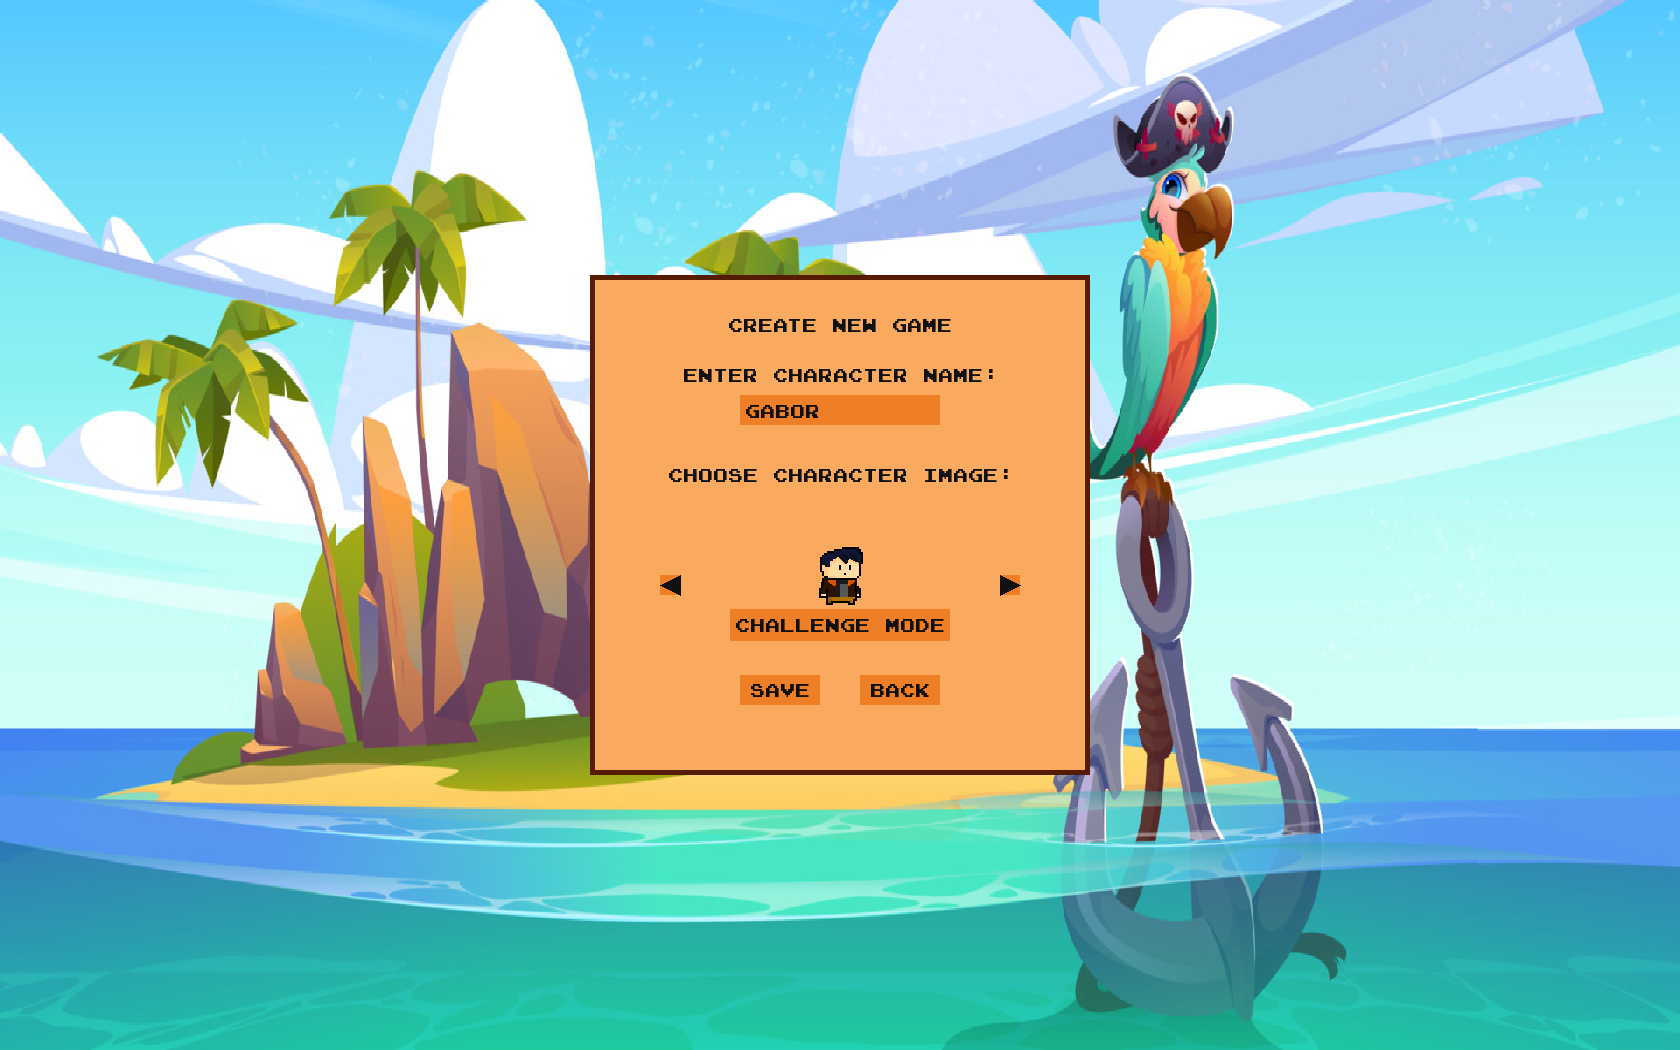
\includegraphics[width=15.0truecm]{images/newgame.png}
    \caption{Új játék létrehozása}
    \label{fig:Új játék létrehozása}
\end{figure}


\subsection{LoadMenu}
A játékosnak lehetősége van a korábban elmentett játékállás betöltésére is, amennyiben van ilyen. A betöltés után a játék folytatódik ahol abbahagyta. Egy lista elrendezésben látja a felhasználó a korábbi mentéseit. Előre rendezi az offline mentéseket a listában, és csak utánuk tölti be az online mentéseket. Egy kattintás után már be is tölti az adott játék állást.


\subsection{GameHandler}
Nagyon fontos szerepet tölt be a játék futása során, ez az osztály kezeli a mentéseket erről a következő szekcióban lesz szó bővebben. 
Továbbá a felhasználói felület kezelése és használata is itt történik. Illetve az összes játékon belüli menü funkció szintén itt példányosodik és van kezelve. Ilyen menük a játékon belüli menü, ami a pillanatálj funkcióval együtt műkdöik, a ranglista, karakter fejlesztési menü, és még az irányítások felület is ahol a felhasználó megtudja nézni, melyik gomb mire való.

\subsection{LevelHandler}
Ez a másik nagyon lényeges osztály, ez a GameHandler-ben kerül példányosításra. Feladata az világok, entitások létrehozása és kezelése. Emellett a kamera kezelés is ide tartozik. 
Ezeket a különböző felületeket Sprite Group-okba szervezve kezeli, így könnyen tudja őket elérni és frissíteni.
Legfontosabb ezek a sprite csoportok közül talán a Visible Sprite csoport, amely a játékos által látható felületeket tartalmazza. A kamera is ezeket rendereli ki, úgy hogy ezeket a csempéket y tengely szerint rendezi és úgy jeleníti meg, ezáltal egy hamis 3D hatást keltve.
Megtalálható még obstacle, attack, és attackable felület csoportok is amelyek a játékmenet során fontos szerepet játszanak, különböző mechanikák végrehajtásánál.


\subsection{Entity}
Ez az osztály egy szülő osztály, ami azt jelenti, hogy ebből származnak le más osztályok és felhasználják minden tulajdonságát illetve metódusait it.  
Három fontos metódussal rendelkezik az egyik a mozgás kezelése, másik egy Sin függvény alapján ad vissza 0-255 értéket, ez később a kapott sebzés kijelzésére szolgál. A harmadik metódus az ütközés érzékelésre, kezelésére szolgál.

Az ütközés érzékelés lényegében úgy műkdöik, hogy nézzük az entitás mozgási irányát függőlegesen, vagy vízszintesen közlekedik, és az adott iránytól függően vizsgáljuk, hogy az entitás hitbox-a ütközik-e valamelyik akadállyal. Ha igen akkor az entitás irány szerinti hitbox-át az akadály ellenkező irányű hitbox-ához igazítjuk, így megakadályozva az áthaladást. (Lásd. 4.2 programkód)
\begin{python}[caption={Ütközés kezelés},label=py:Ütközés kezelés]
    def collision(self, direction):
    if direction == 'horizontal':
    for sprite in self.obstacle_sprites:
    if sprite.hitbox.colliderect(self.hitbox):
    if self.direction.x > 0:
    # moving right
    self.hitbox.right = sprite.hitbox.left
    if self.direction.x < 0:
                        # moving left
                        self.hitbox.left = sprite.hitbox.right
                        
                        if direction == 'vertical':
                        for sprite in self.obstacle_sprites:
                        if sprite.hitbox.colliderect(self.hitbox):
                    if self.direction.y > 0:
                        # moving down
                        self.hitbox.bottom = sprite.hitbox.top
                        if self.direction.y < 0:
                        # moving up
                        self.hitbox.top = sprite.hitbox.bottom
                    \end{python}

A mozgást a move függvény segítségével hajtja végre, amelynek a lényege, hogy az entitás rendelkezik egy irány változóval ami tárolja, hogy merre néz ez lehet (fel, le, jobbra, balra) és ezeknek az irányoknak a normalizálásával és a paraméterként megkapott sebesség értékkel meghatározza a következő pozícióját az entitásnak. Ez a pozíció módosítás a hitbox-ára vonatkozik azaz arra a dobozra amely az entitást körülveszi. Azért a hitbox-ot kell mozgatni, hiszen a szörnyek és karakterek képei a hitboxra vannak igazítva és nem a kép a hitboxhoz. Ez azért fontos mert így megelőzhető az olyan hibák előfordulása, amit a hitbox és a kép közötti eltérés okozhatna.

                    
                    \subsection{Player}
Ez az osztály a játékos karakterét valósítja meg, amely a játék során irányítható. A játékos karaktere egy entitás, így örökli az entitás osztály összes tulajdonságát és metódusát. Az osztály inicializálása során számos fontos adatot tárol, például a játékos nevét, karakterének azonosítóját és kezdeti pozícióját. Ezek az adatok meghatározzák a karakter kezdeti állapotát a játékban. A karakter mozgását és irányítását az osztály input metódusa kezeli. Ennek segítségével az osztály figyeli, hogy milyen billentyűk vannak lenyomva, és ennek megfelelően mozgatja a karaktert a játékban. A játékos karakter képes balra, jobbra, felfelé és lefelé mozogni a megfelelő billentyűk lenyomásával. A karakter sebessége és energiaszintje dinamikusan változik a játék során. Például a karakter gyorsabban mozoghat, ha lenyomja a "SHIFT" billentyűt, és az energia szintje csökken mindeközben. Az energia idővel regenerálódik, ami lehetővé teszi, hogy tovább használhassa a gyors futás funkciót. A játékos karakter képes támadni is, és az attack metódus meghívásával hozza létre a támadást. A támadásokat az osztály figyeli, és számítja ki a támadások közöt eltelt időt, hogy ne lehessen túl gyorsan ütni a fegyverekkel. A karakter fegyvere is dinamikusan változik, és a játékos lehetőséget kap a fegyver cseréjére a játék során. A karakternek vannak életpontjai és energia szintje, amelyek határozzák meg túlélését a játékban. Amennyiben az életpontja nullára csökken, a karakter meghal, de van lehetőség a visszatérésre vagy újrakezdésre a játékban, attól függően, hogy milyes a játék nehézségi szintje. A karakter számos egyéb tulajdonsággal és képességgel rendelkezik, például tapasztalati pontokkal, megszerzett arany mennyiségével és teljesített küldetésekkel. Ezek a tényezők befolyásolják a játékmenetet és a karakter fejlődését. Az osztály továbbá lehetővé teszi a karakternek, hogy tárgyakat használjon és rendelkezzen egy táskával. A játékos képes tárgyakat váltani és használni a játék során, ami további taktikai elemet ad a játékhoz. Összességében ez az osztály kulcsfontosságú a játékos karakter kezelésében és irányításában, lehetővé téve a játékosnak, hogy részt vegyen a játék világában és kihívásokkal nézzen szembe a karaktere fejlesztése során.
\subsection{World, Dungeon}

Egy közös szülő osztályból származnak le, ez azért fontos, hogy a különböző világokat könnyen tudjam kezelni és különböző tulajdonságokat adni nekik. Ebben az osztályban a minden világra vonatkozó lehetőségeket kezelem, ilyen például az effekteket lejátszó AnimationPlayer osztályom származtatása, hiszen azt elég egyszer definiálni és felhívni ott ahol szükséges ahelyett, hogy minden világnak lenne egy külön példánya. Továbbá ilyen opció a térképmegnyitás, és az azzal kapcsolatos összes funkció, hol található a következő küldést adó nem játékos karakter. Hiszen a játék története jelenleg teljesen lineáris, tehát egy adott sorrendben történhet csak a küldetések teljesítése. Amit még fontos megemlíteni ezzel az osztállyal kapcsolatban, az a szörnyek által dobott tárgyak, ilyen tárgy jelenleg, a tapasztalati pont, és az aranypénz. Ezeket a tárgyakat a játékos fel tudja venni, és a játék során fel tudja használni.  

\subsubsection{Pálya generáláshoz szükséges adatok}

Említettem a korábbi fejezetben, a pálya megtervezését a \textbf{Tiled}-el végeztem. (Lásd \ref{subsec:Tiled}) 
Első megközelítésemkor CSV (vesszővel elválaszott értékek) fájl formátumba mentettem ki a tervezőben létrehozott rétegeket. Egy ilyen dokumentum úgy néz ki, hogy ahova nem helyeztem le a tervezőben objektumot ott '-1' érték szerepel, ellentétben ahol van érték ott a Tiled-ben betöltött és feldarabolt csempekészlet azonosító számai kerültek a dokumentumba. Ezt úgy kell elképzelni mint egy nagy mátrixot. Az utolsó pillanatokig ezt a megközelítést alkalmaztam, hiszen ha már kész volt és működött miért változtattam volna rajta. Végül mégis visszatértem erre a kérdéskörre és készítettem az alább olvasható kis egyszerű átalakító szkriptet. (Lásd \ref{py:csvtodict}) Ennek funkciója, a sok felesleges '-1' értéket kiszűrni, hogy a program futása közben, ne kelljen a betöltésnél rengeteg felesleges összehasonlítást végezni. Ezt úgy oldottam meg, hogy készítettem python szótárat a csempe azonosító számából illetve annak a csv mátrixban elhelyezkedő koordinátáiról. (Lásd \ref{py:átalakított struktúra})


\begin{python}[caption={csvtodict},label=py:csvtodict]
    import csv
    import json
    
    csv_file = "new_map\MSmap._dungeonentrance.csv"
    map_data = []
    
    with open(csv_file, newline='') as csvfile:
        csv_reader = csv.reader(csvfile)
    
        for i, row in enumerate(csv_reader):
            for j, value in enumerate(row):
    
                value = int(value)
    
                    map_data.append({"i": i, "j": j, "value": value})
    
    python_file = "world_dungeonentrance"
    
    with open(python_file, 'w') as pyfile:
        pyfile.write("map_data = ")
        json.dump(map_data, pyfile, indent=4)
    
    print(f"Dictionary saved to {python_file}")
    
\end{python}


\begin{python}[caption={Minta az átalakított struktúrára}, label=py:átalakított struktúra]
    {
        "i": 3,
        "j": 41,
        "value": 125
    },
\end{python}


\subsubsection{Pálya generálás}

Most, hogy már grafika és a pálya rétegek elkészültek amik ki lettek exportálva, ideje ezeket az adatokat egyesíteni és megjeleníteni a játékban. Ezt több lépésben valósítottam meg, először is a képeket be kell tudnom olvasni, ezt az os könyvtár walk függvényének segítségével oldottam meg. Miután sikerült bejárni a mappát, előállítom az egyes képekhez vezető útvonalat, és ezután a pygame.image.load függvényével betöltöm a képeket. Ezt követően a képeket egy listába helyezem, amelyet később fel tudok használni a kirajzoláshoz. Másik ilyen fontos lépés a pálya rétegek beolvasása, amelyet a korábban említett szótárak segítségével valósítottam meg. Ezután egy ciklusban végig iterálva a szótáron, a képek listájából kiválasztom a megfelelő képet, és a megfelelő koordinátákat amiket segítségével példányosítom a Tile (csempe) osztályt később ennek segítségével végzem el a kirajzolást. Mivel a szótárak között szerepel az entitásokra vonatkozó réteg is, ezért azokat is az előbb említett iterációban kezelem, és példányosítom a hozzájuk tartozó osztályokat azonosító alapján szűrve.

Készítettem egy kis függvényt, a pálya létrehozásának idejének meghatározására. Ez azért volt fontos, hogy megtudjam határozni, hogy a szótár használata jobb megoldás-e, mint a CSV fájl. A két megoldás esetében a következő eredményeket kaptam:

Szótár esetében:
\begin{verbatim}
    Futási idő: 108.64 ms
\end{verbatim}
CSV fájl esetében:
\begin{verbatim}
    Futási idő: 879.92 ms
\end{verbatim}

Tehát elmondható, hogy ez a változtatás jelentősen felgyorsította a pálya létrehozását, ezáltal a játék betöltési ideje is csökkent.

\subsection{Enemy}

Az ellenségek a játékban a küldetések után talán a legfontosabb mechanikái a játknak, hiszen a velük való harc kiemelt szerepet kap a történet során.
Az ellenségek is egy közös szülő osztályból származnak le, ez azért volt fontos, hogy a különböző ellenségeknek különböző tulajdonságokat tudjak adni. Például a sebesség, életerő, támadási sebesség, támadások hangjai. Ezeket a tulajdonságokat settings statikus osztály monster\_data dictionary-ben tárolom és olvasom be.

A szörnyek mozgását úgy valósítottam meg, hogy ha a játékos egy adott sugaron belül ér a szörnyhöz képest ez az úgynevezett érzékelési sugár akkor kiszámolom vektorokkal a játékos távolságát és ha a távolság nagyobb mint 0 azaz nem egy helyen állnak, akkor meghatározom az irányt a két vektor különbségének normalizálásával. A távolság érték azért fontos, hogy megállíptsa mikor ér a játékos karaktere a szörnyhöz támadási távolságon belülre. Az irány érték pedig a szörny mozgatásához szükséges.

Három különböző státusszal rendelkezhet egy ellenség. Támadási státuszt kap ha támadási sugaron belül tartózkodik a játékos karaktere, és ha egy bizonyos idő eltelt az előző támadás óta. Mozgás státuszt kap ha a játékos karaktere a szörny érzékelési sugarán belül van, de nem támadási sugaron belül. Ha a játékos karaktere nincs az érzékelési sugarán belül akkor pedig nyugalmi státuszt kap. Ezek a státuszok határozzák meg a szörnyek viselkedését és a megjelenített grafikát is a játék során.


\subsection{NPC}

Nem játékos által vezértelt karakterek azaz NPC-k egy kalandjáték során elengedhetetlen részei a történetnek és a játékmenetnek. Ahogy az összes többi szörny, játkos osztály is az Entity osztályból származik le, hiszen adott esetben szükség lehet mozgatásra és ütközés érzékelésre. Azonban a legtöbb esetben a játékos karaktere nem tudja megölni ezeket az entitásokat, hiszen a történet során szükség van rájuk. Ezért a játékos karaktere nem tud ütközni velük, és a szörnyekkel ellentétben nem tudnak támadni.

\subsection{Questgiver}

A játékom egyik legfontosabb mechanikája a küldetés rendszer, hiszen ezen alapszik az előrehaladás illetve a challange játékmódnál az újraindítás is a küldetések teljesítését érzékelve valósul meg. 

A Questgiver NPC típúst a World osztály példányosítja és a példányok osztályváltozóinak inicializálásakor olvassa be a saját id-jéhez tartozó küldetéseket a Settings osztály npc\_data dictionary-jéből. Majd ezt követően a World osztály létrehozz a Player osztályból is egy példányt amely egészen a LevelHandler osztálytól kap paraméterként egy questgivers\_quest\_setup függvényt, amely egy trigger után vizsgálja hogy a játékos álltal már teljesített küldetés szerepel\-e még Questgivernél és, ha igen akkor kitörli azt. Ezáltal elkerülhető a küldetés ismétlődése. Küldetést nem lehet kihagyni mindegyiket sorban kell teljesíteni, ahogy a történet halad előre.

Az questgiver típúsú NPC-k képesek egy előre megírt dialógus megjelenítésére (Lásd. 4.5 ábra), amelyben a játékos választhat két lehetőség közül amelyek a küldetés elfogadása vagy elutasítása. A választás megerősítése történhet a kurzornak a gomb felé mozgatásával ezután egy kattintással, vagy a billentyűzet segítségével egyaránt. A dialógus ablak megnyitásához szükséges a játékos karakteréhez viszonyított távolság érzékelése, hiszen egy beszélgetés során közel kell állni a kommunikációban résztvevő többi szereplőhöz ezt hasonló módon vizsgálom, mint ahogy a szörnyek esetében az érzékelési távolságot vizsgáltam. Illetve dialógus megjelenítéséhez még szükséges, hogy az adott NPC rendelkezzen a soron következő küldetés azonosítójával is.   

\begin{figure}[H]
    \centering
    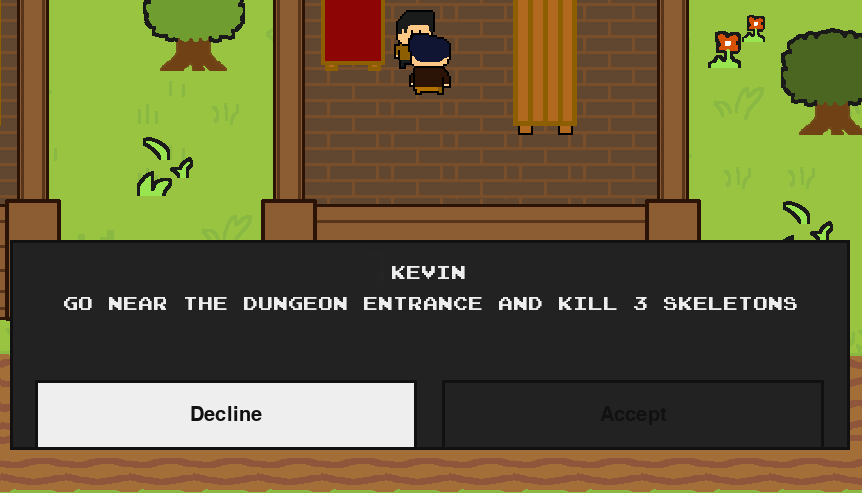
\includegraphics[width=14.0truecm]{images/dialogue.png}
    \caption{Dialógus}
    \label{fig:Dialógus}
\end{figure}

\subsection{Merchant}

Egy kalandjátékban az előrehaladás mellett fontos, hogy a nehezen megszerzett tárgyakkal, esetünkben az arannyal lehessen mit kezdeni, ezért egy Merchant NPC típús létrehozását láttam a legjobb ötletnek, hiszen rengeteg különböző módon fellehet őket használni. 

Egyenlőre csak bájital árusításra szolgáló merchant van a játékban (élet visszatöltő, energiát növelő, sebzést növelő bájitalok árusítására szolgál). A továbbfejleszétsi lehetőségek bekezdésben jobban kifejtem mikre lehet még használni a merchant típúsú NPC-t.  Ahogyan a Questgivernél is itt is a távolságvizsgálat alapján és egy gomb lenyomására történik a vásárlásra szolgáló ablak megjelenítése (Lásd. 4.6 ábra). A vásárlás során a játékos karakterének az egyenlege/arany mennyisége csökken, és a vásárolt tárgyak a hátizsákjába kerülnek.

Azt, hogy milyen tárgyakat adhat el egy bizonyos merchant azt a Settings osztályból egy dictionaryben tárolt id-k beolvasása befolyásolja. Illetve a Settings osztály tartalmaz egy Items dictionary-t is amelyben a tárgyakra vonatkozó adatokat tárolom. Ilyen adatok például a tárgy neve, típúsa, ára hatása és annak mennyisége (Például mennyi plusz erő-t ad a tárgy), illetve a időtartamra vonatkozó megkötést és talán a legfontosabbat a grafikának az elérési útvonalát.  

\begin{figure}[H]
    \centering
    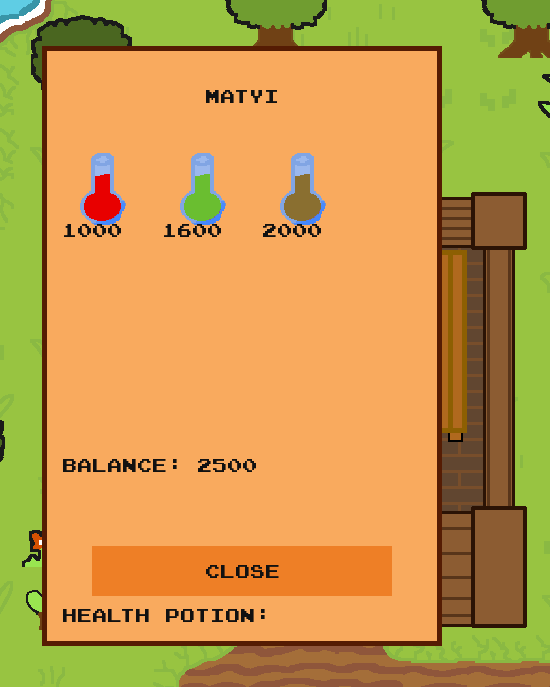
\includegraphics[width=9.0truecm]{images/merchant.png}
    \caption{Merchant}
    \label{fig:Merchant}
\end{figure}


\subsection{inventory}

Inventory azaz táska rendszer, fontos szerepet kap a játék folyamán hiszen a merchanttól megvásárolt tárgyak ebbe a hátizsákba kerülnek bele és a játékos ezeket felhasználni amikor szükségét érzi.

Öt szabad férőhellyel rendelkezik a táska ezért jól meg kell válogatni mik azok a fontos tárgyak amelyeket oda szeretne helyezni a játékos. Első nekifutásra egy futószalag szerű működést képzeltem el a táska rendszernek, amelyet azért gondoltam jó ötletnek, mert a megvalósítása egyszerű volt, hiszen megszerzett tárgyak időrendben kerültek bele a táskába. Viszont felvetette a problémát, hogy ha más sorrendben esik kézre a felhasználónak, vagy nincs helye akkor mit tud tenni. Ezért úgy döntöttünk, hogy jobb megoldás lenne, ha az azonos tárgyakkat össze lehetne húzni egy férőhelyre, ezáltal kényelmesebbé válna a használata a táskának. Megtartottam a futószalag szerű megoldást, viszont kiegészült a tárgy összevonással amelyet egy számláló bevezetésével oldottam meg, amely jelzi a felhasználónak, hogy még mennyi található nála abból az adott tárgyból. (Lásd. 4.7 ábra)

\begin{figure}[H]
    \centering
    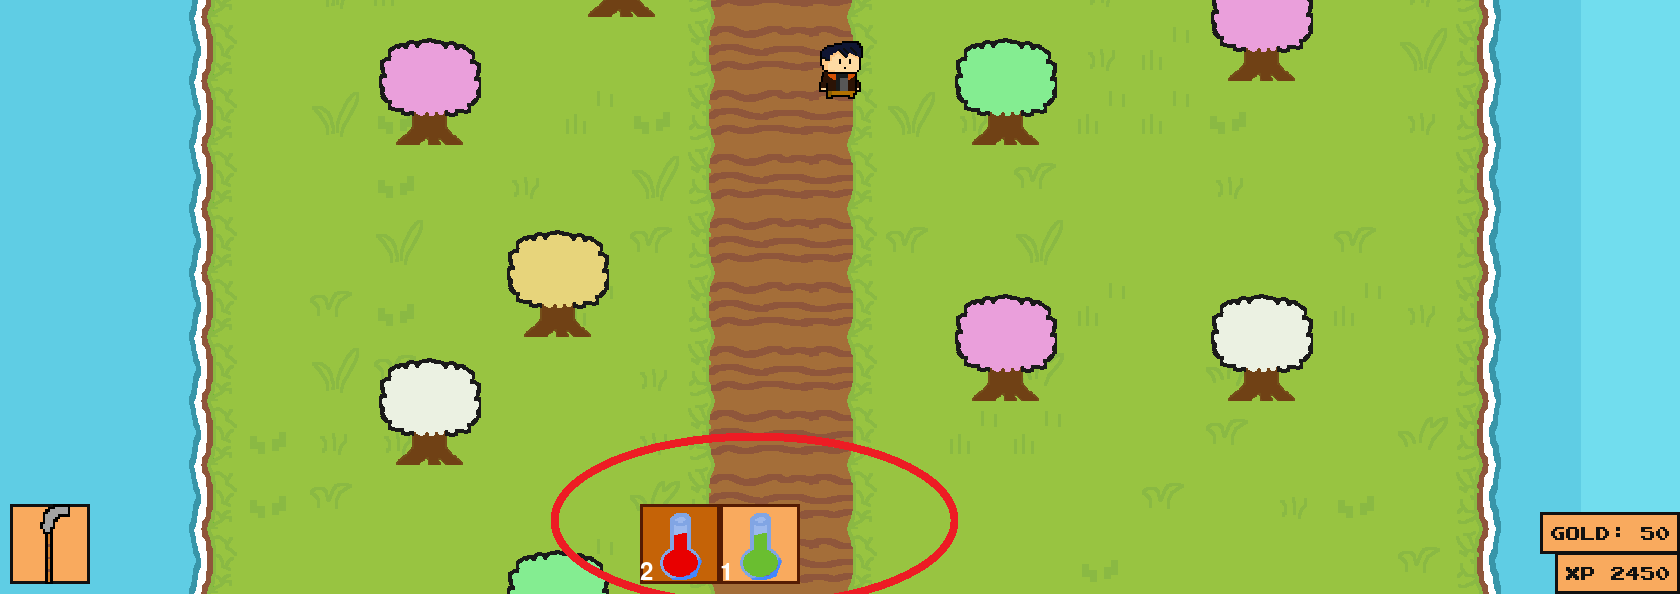
\includegraphics[width=15.5truecm]{images/inventory.png}
    \caption{Táksa rendszer}
    \label{fig:Táska rendszer}
\end{figure}

\subsection{Loot}

A zsákmányolás funkciót azért tartottam fontosnak, hiszen plusz motivációt nyújt a játékosnak legyőzni a szörnyeket, ha szerezhet is tőlük tárgyakat. Egyenlőre a szörnyek három különböző tárgy dobására képesek. Tapasztalati pont bogyókat hagynak hátra, amelyek előre meghatározott mennyiségű tapasztalati pontot tartalmaznak, és mindegyik szörny ilyet hagy maga után a legyőzése után. Ezenkívül aranyat is dobhatnak, két különböző fajtát, bár erre már nem minden szörny képes, és ez ritkábban fordul elő. Az egyik fajta kis mennyiségű aranyat tartalmaz, míg a másik nagyobb mennyiségű aranyat ad. 

A drop\_loot függvényt a szörnyek példányosításkor paraméterként megkapják és, ha elfogy az életpontjuk akkor hívják meg azt. Ez a metódus meghatároz a szörny legutóbbi pozíciójához viszonyítva egy 100x100-as négyzeten belüli pozíciót ahova a zsákmányolható tárgyak kerülni fognak. Ezt követően a szörny típúsához viszonyítva kiolvassa a Settings osztály monster\_data dictionary-jéből, hogy az adott szörny milyen tárgyakat dobhat, majd ez alapján az előre meghatározott esély alapján véletlenszám generálásával eldönti, hogy milyen tárgyakat hoz létre. A létrehozás úgy történik, hogy az adott pálya példánynak a loots osztályváltozójához hozzá fűz egy Loot osztály példányát amely tárgy nevét, mértékét, és helyét.

A kirajzolása a felvehető tárgyaknak a visible sprite csoport frissítésével történik, hiszen a Loots osztály ahogy a többi objektum is, a pygame.sprite.Sprite osztályból származik le.  

Tárgyak felvétele a tárgy pozíciója és a játékos karakternéket távolságát vizsgálva történik, ha elég közel megy a játékos a tárgyhoz akkor kitörli a kitörli a loots listából a felvett tárgyat és az értékeit hozzáadja a játékos karakterének a tulajdonságaiban tárolt értékekhez.

\begin{figure}[H]
    \centering
    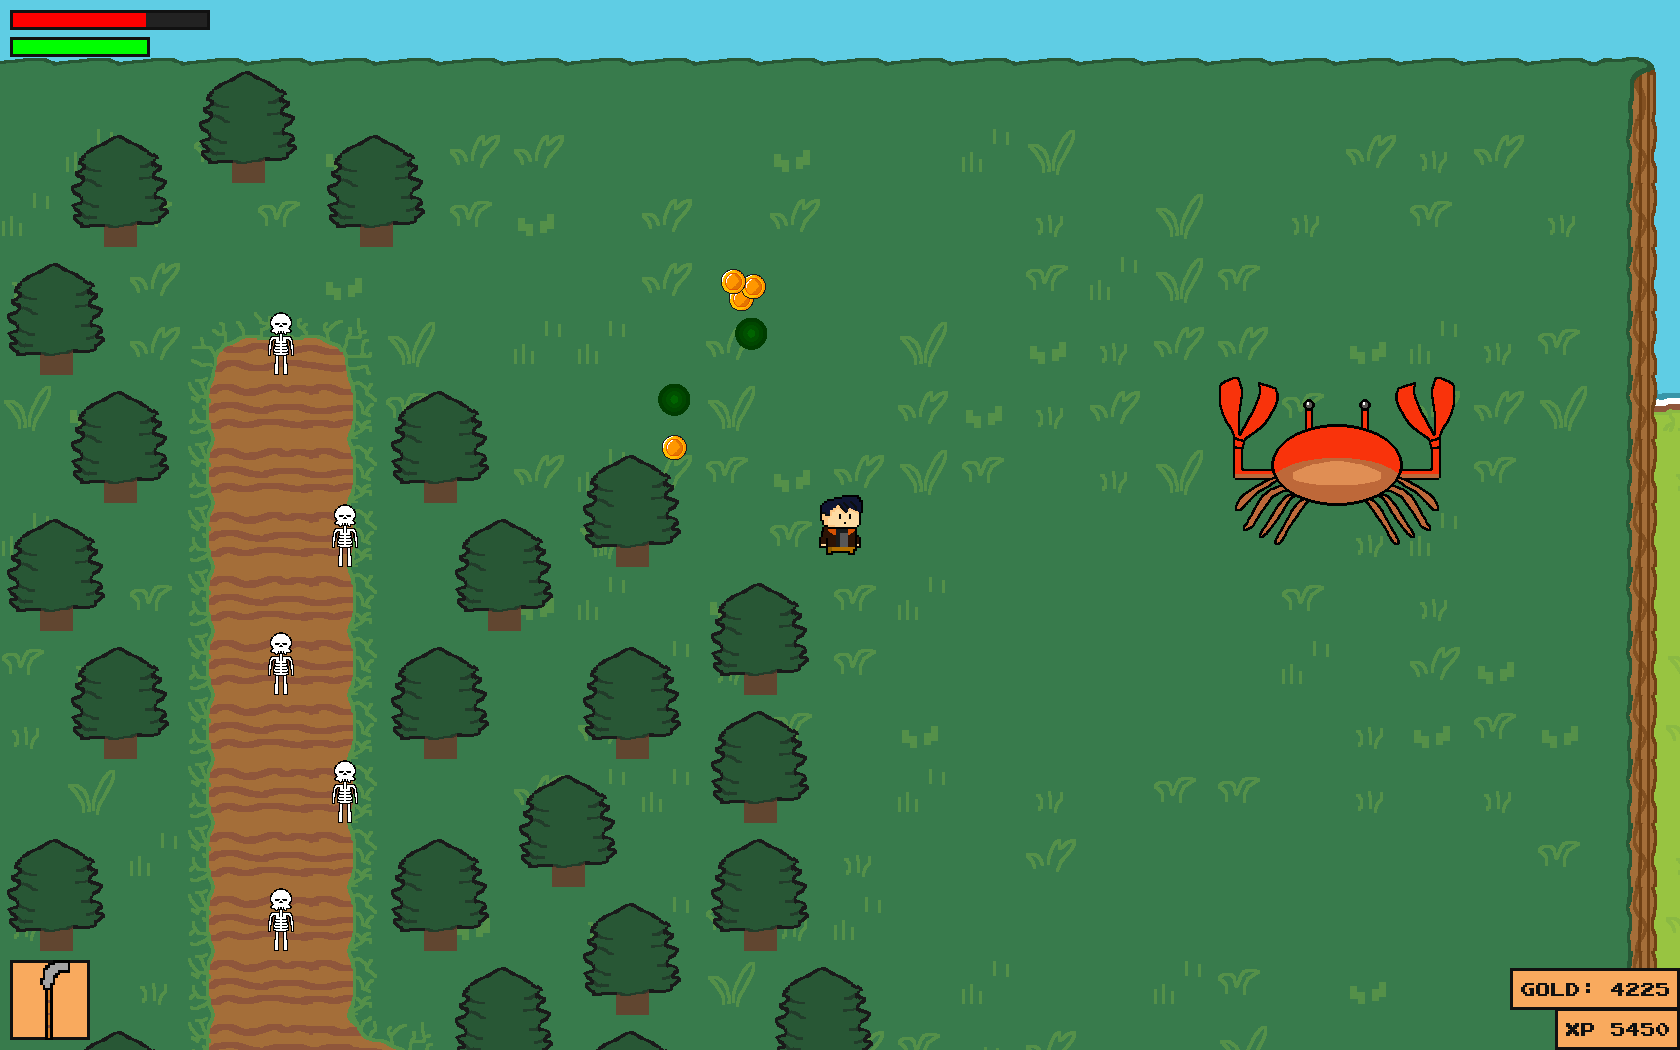
\includegraphics[width=15.5truecm]{images/loots.png}
    \caption{Zsákmányolás funkció}
    \label{fig:Zsákmányolás funkció}
\end{figure}


\subsection{Weapon}

A különböző fegyverek használata szintén egy elengedhetetlen része lett a játéknak. A fegyvereket a játékos karaktere használja a szörnyek elleni harc során. 

Ezen harcolásra szolgáló eszközök kirajzolása a támadás gomb lenyomása után történik a Weapon osztály példányosításával. Ez az osztály a játékos karaktere által kezében tartott fegyver rajzolja ki a képernyőre. Mivel fontosnak tartottam, hogy mozgás közben is lehessen támadni, illetve legyen egy csapás/suhintás animáció ezért egy frissités funkciót vezettem be, amely mindig a játékos karakterének legutóbbi helyzetét, és irányát vizsgálja majd ezekre az adatokra alapozva frissíti a már létrehozott felületet. A csapás animációt mind a négy irányban külön-külön kellett megtervezni, hiszen a fegyverek nem egyformán néznek ki minden irányból. Sinus függvény segítségével valósítottam meg a megjelenített fegyver forgatását egy amplitúdó értékkel amely a fegyver típusától függően változhat.

Ahogyan a többi látható objektum ezek a fegyverek is a visible sprite csoport része, viszont rendelekzik az attack\_sprites csoporttal is amely segít megkülönböztetni a többi felülettől a fegyvereket, ezáltal támogatva a támadási logika megvalósítását. A támadási logika egy metódus, amely ezeken az attack\_sprites csoporton végig iterál, és vizsgálja az attackable\_sprites felületekkel való ütközést amelyeket olyan entitások kaphatnak, amelyekkel a játékos meg tud küzdeni a játék során, legyen az egy szörny vagy akár egy kiüthető fűcsomó.  

\begin{figure}[H]
    \centering
    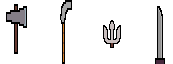
\includegraphics[width=15.5truecm]{images/weapons.png}
    \caption{A játékban megtalálható fegyverek}
    \label{fig:A játékban megtalálható fegyverek}
\end{figure}


\subsection{ingame\_menu}

Játékmenet közbeni menü amely lehetővé teszi a játékállapot mentését kezelő metódus elindítását a Save gomb megnyomásával és egyben egy pillanatálj funkció elérését is. 

A pillanatálj funkciót úgy valósítottam meg, hogy az összes játékbeli sprite group azaz felületi csoport kirajzolására szolgáló függvényt állítom le egy boolean típúsú változóval ezáltal minden játékon belüli elem megáll a legutolsó ismert állapotában, majd a menü bezárása után, amelyet a resume gomb megnyomásával tehet meg a játékos, onnan folytatódnak az események ahol abbamaradtak.

\subsection{Save}

Ahogy a korábbi fejezetekben már említettem a játékállapot mentését a Save gomb megnyomásával lehet elérni. A mentés a játékállapot minden fontosabb elemét eltárolja egy JSON típúsú fájlban, ha offline módban játszik a játékos, vagy FastAPI-n keresztül kommunikálva egy mysql adatbázisban, ha online módot választott a felhasználó.


\section{Adatbázis használata a programban}

Az online mentés kezeléséhez, illetve a játékban való regisztrációhoz és bejelentkezéshez szükség volt egy backend megvalósítására azaz egy alkalmazásra amely kommunikációt végez az adatbázissal. Ezt a FastAPI nevű python könyvtár segítségével valósítottam meg. A FastAPI egy modern, gyors, könnyű keretrendszer a microservice-ekhez talán a legjobb választás python programozási nyelv esetében.

Az adatokat különböző requestek és a megfelelő URL segítségével tudjuk elérni, vagy adott esetben felvinni, frissíteni. A FastAPI érzékeli, hogy egy kéérés érkezett a rendszerbe, és ha az adott kérés teljesíthető akkor az esetemben megkezdi a kommunikációt a mysql adatbázissal és a visszakapott adatokat BaseModell típusú objektumokba tölti, amelyeket a Pydantic könyvtár segítségével tudok kezelni. Ez a modell azért fontos mert validálja, hogy a kérésben szereplő adatok megfelelnek-e a megadott adatstruktúrának. Miután a validálás is sikeresen lezajlott a FastAPI visszaküldi a végpont kérésre a megfelelő választ.

